\chapter{Introduction}


\section{mRNA Life Cycle}

Transcription is the first step in gene expression in which a premature RNA
    molecule is made from a gene's DNA template.
In eukaryotes, splicing, adding a 5' cap and poly-A-tail, as well as binding of cap-
    and RNA-binding proteins yields mature messenger RNAs (mRNAs).
These mRNAs are then typically exported through nuclear pore complexes, which perforate the
    nuclear envelope.
Once in the cytoplasm, the acquired protein coat determines the fate of the mRNA \cite{moore_birth_2005}.
Translation, a process involving polysome assembly and protein coat remodeling,
    can occur immediately or delayed, such as in the case of various developmental
    transcripts.
After translation is arrested, polysomes get disassembled and mRNAs are deadenylated.
    mRNAs can now be degraded or stored until internal or external signals call for
    their renewed translation.
Subsets of these mRNAs can be packaged into RNA granules (Figure \ref{fig:introduction}A).
RNA granules are cytoplasmic, membrane-less aggregates containing 
    various proteins involved in translation initiation and repression (reviewed in \cite{anderson_rna_2006}).

\begin{figure}[b!]
    \centering
    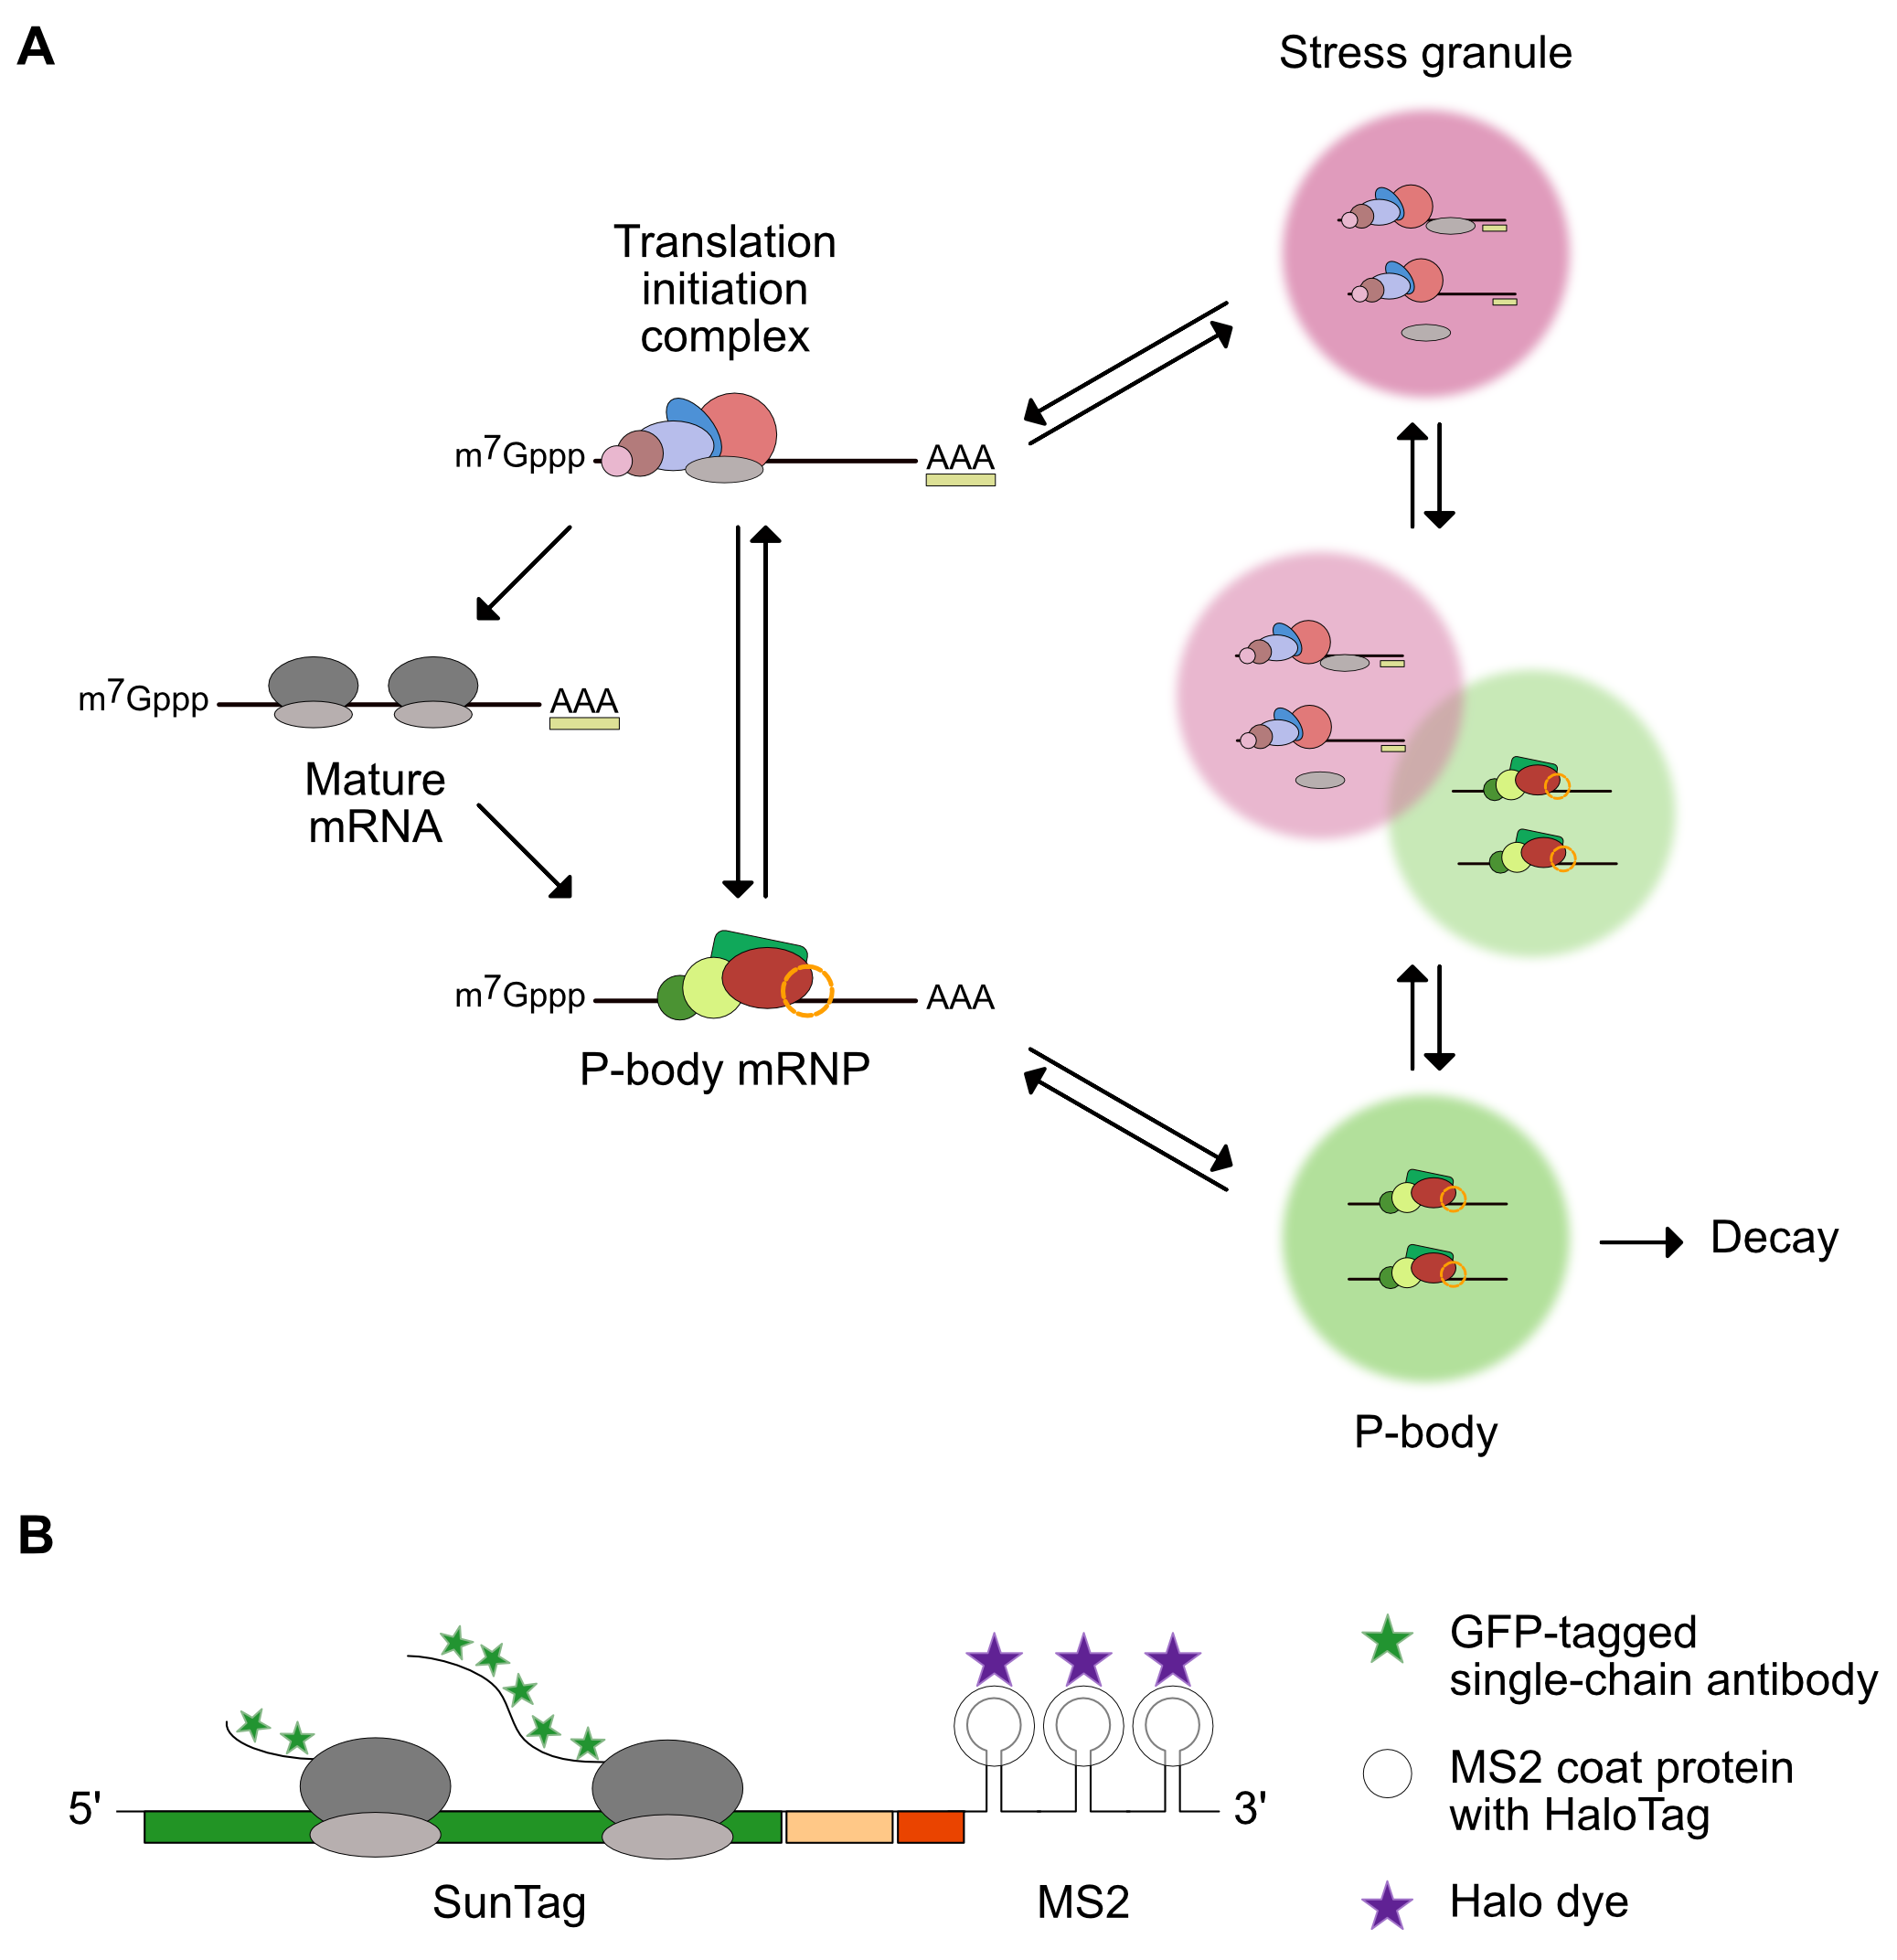
\includegraphics[width=\linewidth]{images/figure1}
    \caption{\textbf{mRNA life cycle and translation site imaging.}
        (A) Overview of a typical mRNAs life cycle ranging from
            translation to decay.
        (B) Schematic description of SunTag imaging to visualize and quantify
            translational activity on single-molecule level.
    }
    \label{fig:introduction}
\end{figure}

Stress granules (SGs) are a prominent type of RNA granules that exclusively form
    under stress.
Consensus suggests that, due to their enrichment in initiation factors,
    SGs exclusively contain translationally repressed mRNAs (reviewed in \cite{thomas_rna_2011}).
However, recent findings have reported otherwise \cite{mateju_single-molecule_2020}.
While SG formation seems to be a conserved phenomenon throughout eukaryotes,
    their function remains unclear.
SG formation was found to involve the nucleation through translationally silent messenger ribonucleoproteins (mRNPs).
Proteins such as T-cell intracellular antigen-1 (TIA-1) \cite{kedersha_rna-binding_1999} and Ras GTPase-Activating Protein-Binding
    Protein 1 (G3BP1) \cite{tourriere_rasgap-associated_2003} have been found to induce SG formation upon overexpression.

mRNA Processing Bodies (P-bodies) were originally described as mouse XRN1p
    (a highly conserved 5'-3' exonuclease) foci in the cytoplasm \cite{bashkirov_mouse_1997}.
P-bodies, unlike stress granules, are present in unstressed physiology.
However, stress can further increase their formation (reviewed in \cite{parker_p_2007}).
Beside co-translational mRNA decay through various RNases, P-bodies are considered one
    of the main sites of mRNA degradation.

\section{Translation Site Imaging} \label{translation_site_imaging}

To better understand the translational dynamics of single transcripts, a recent
    method has emerged.
The stellar explosion supernova (SunTag) imaging approach allows for live-cell imaging-based analysis to visualize and
    quantify translation sites \cite{tanenbaum_protein-tagging_2014}.
The SunTag system relies on three core components: a reporter RNA containing a SunTag 
    cassette and MS2 stem-loops, a GFP-tagged single-chain antibody (scAB) against GCN4,
    and an MS2 coat protein fused to a HaloTag (Figure \ref{fig:introduction}B).
Currently available standard SunTag cassettes consist of 24 GCN4 repeats that, upon translation
    and exposure of the GCN4 epitopes, can be recognized and bound by the co-expressed scAB.
As translation continues, more epitopes get revealed allowing more scABs to bind.
This increases the local GFP concentration and thereby brightens the fluorescent signal.
The MS2 coat protein-HaloTag fustion in conjunction with a soluble Halo dye is used
    to visualize the MS2 stem loops on the reporter RNA.
Taken together, the system allows for accurate tracking of single RNAs and simultaeous
    brightness-inferred translational quantification.
